\documentclass{beamer}
\usetheme{Madrid}
\usecolortheme{default}

\usepackage{amsmath,amssymb,amsfonts}
\usepackage{graphicx}
\usepackage{xcolor}
\usepackage{listings}

% Listings style
\lstset{
  language=C,
  basicstyle=\ttfamily\small,
  keywordstyle=\color{blue},
  commentstyle=\color{gray},
  stringstyle=\color{red!60!black},
  showstringspaces=false,
  breaklines=true,
  frame=single,
  numbers=left,
  numberstyle=\tiny,
  stepnumber=1,
  numbersep=6pt,
  tabsize=2
}

% Custom macros
\newcommand{\myvec}[1]{\begin{pmatrix}#1\end{pmatrix}}
\newcommand{\brak}[1]{\left( #1 \right)}

% Redefine \vec to bold letters only (no arrow)
\renewcommand{\vec}[1]{\mathbf{#1}}

\title{2.7.31}
\author{EE25BTECH11019 - Darji Vivek M.}
\date{}

\begin{document}
\frame{\titlepage}

% Question Frame
\begin{frame}{Question}
Find the area of triangle $ABC$, whose vertices are
\[
A(2,5), \quad B(4,7), \quad C(6,2).
\]
\hfill (12, 2018)
\end{frame}

% Variables Frame
\begin{frame}{Given Data}
\[
\vec{A} = \begin{bmatrix}2\\5\end{bmatrix}, \quad 
\vec{B} = \begin{bmatrix}4\\7\end{bmatrix}, \quad 
\vec{C} = \begin{bmatrix}6\\2\end{bmatrix}
\]
\[
\vec{A}-\vec{B}=\begin{bmatrix}-2\\-2\end{bmatrix},\quad 
\vec{A}-\vec{C}=\begin{bmatrix}-4\\3\end{bmatrix}
\]
\end{frame}

% Solution Frame
\begin{frame}{Solution}
Area of triangle \(ABC\):

\[
\Delta \;=\; \frac{1}{2}\,\big|(\vec{A}-\vec{B})_1(\vec{A}-\vec{C})_2
    - (\vec{A}-\vec{B})_2(\vec{A}-\vec{C})_1\big|.
\]

Substitute \((\vec{A}-\vec{B}) = (-2,-2)\) and \((\vec{A}-\vec{C}) = (-4,3)\):
\[
\Delta = \frac{1}{2}\,\big|(-2)(3) - (-2)(-4)\big|
       = \frac{1}{2}\,\big|-6 - 8\big|
       = \frac{1}{2}\cdot 14 = 7.
\]

\[
\therefore \quad \text{Area of } \triangle ABC = 7.
\]
\end{frame}

% C Code Frame (inline)
\begin{frame}[fragile]{C Code Implementation}
\begin{lstlisting}
#include <stdio.h>
#include <math.h>

// Function to compute area of triangle from 3 points
double triangle_area(double x1, double y1,
                     double x2, double y2,
                     double x3, double y3) {
    double det = x1*(y2 - y3) - y1*(x2 - x3) + (x2*y3 - y2*x3);
    return fabs(det) / 2.0;
}
\end{lstlisting}
\end{frame}
\begin{frame}[fragile]{C Code Implementation}
\begin{lstlisting}
int main() {
    double A[2] = {2, 5};
    double B[2] = {4, 7};
    double C[2] = {6, 2};

    double area = triangle_area(A[0], A[1], B[0], B[1], C[0], C[1]);
    printf("Area of triangle ABC = %.2f\n", area);
    return 0;
}
\end{lstlisting}
\end{frame}

\begin{frame}[fragile]{Python code}
\begin{lstlisting}
import numpy as np
import matplotlib.pyplot as plt

# Points
A = np.array([2, 5])
B = np.array([4, 7])
C = np.array([6, 2])

# Area using determinant method
matrix = np.array([
    [A[0], A[1], 1],
    [B[0], B[1], 1],
    [C[0], C[1], 1]
])
area = 0.5 * abs(np.linalg.det(matrix))
print(f"Area of triangle ABC = {area:.2f}")
\end{lstlisting}
\end{frame}

\begin{frame}[fragile]{Python code}
\begin{lstlisting}
# Plot triangle
x_coords = [A[0], B[0], C[0], A[0]]
y_coords = [A[1], B[1], C[1], A[1]]

plt.plot(x_coords, y_coords, 'b-', label='Triangle ABC')
plt.scatter([A[0], B[0], C[0]], [A[1], B[1], C[1]], color='red')

# Annotate points
labels = ['A(2,5)', 'B(4,7)', 'C(6,2)']
for (x, y), label in zip([A, B, C], labels):
    plt.annotate(label, (x, y), textcoords="offset points", xytext=(5,5), ha='center')
\end{lstlisting}
\end{frame}

\begin{frame}[fragile]{Python code(plots)}
\begin{lstlisting}
plt.title("Triangle ABC")
plt.xlabel("x")
plt.ylabel("y")
plt.grid(True)
plt.axis('equal')
plt.legend()
plt.savefig("triangle.png")
plt.show()

\end{lstlisting}
\end{frame}

\begin{frame}{Python Output and Plot}
\begin{figure}[h!]
\centering
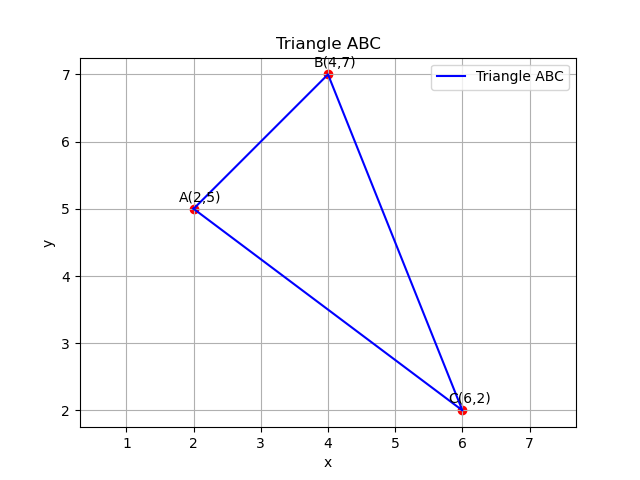
\includegraphics[width=0.75\columnwidth]{figs/triangle.png}
\caption{Triangle $ABC$ with vertices A(2,5), B(4,7), C(6,2)}
\end{figure}
\end{frame}

\end{document}
